\section{Algoritmos y aplicaciones}
Dado el problema planteado, su solución implica el uso de algoritmos de visión por computadora.

\subsection{Redes neuronales convolucionales (CNN)}
Las redes neuronales convolucionales (CNN) son una alternativa especialmente adecuada para este problema debido a su capacidad para procesar información espacial. Mediante filtros convolucionales pueden aprender automáticamente características de las imágenes, como bordes, texturas y formas (Figura~\ref{fig:cnn_diagram}). En las capas internas pueden emplearse funciones de activación como ReLU, mientras que Softmax puede utilizarse en la salida para representar las probabilidades de las distintas clases.

\begin{figure}[pos=!ht]
    \centering
    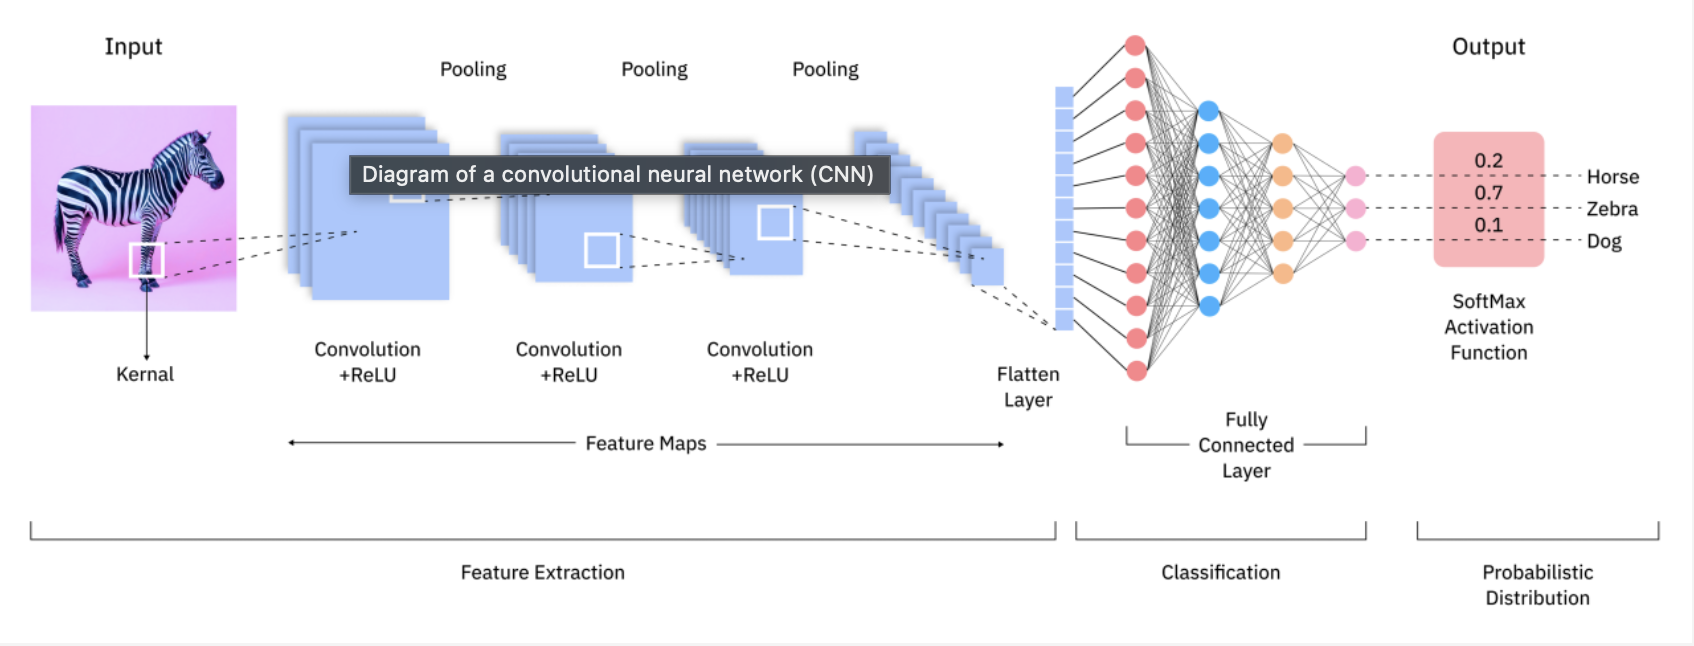
\includegraphics[width=\columnwidth]{cnn_diagram.png}
    \caption{La convolución descompone la imagen en características para aprender a clasificar \parencite{ibmWhatImage}.}
    \label{fig:cnn_diagram}
\end{figure}

Este método parece ser el más adecuado para obtener buenos resultados; sin embargo, por la cantidad de datos y de operaciones involucradas, es lento y computacionalmente pesado. Esto abre la posibilidad de usar otros algoritmos que se ajusten a las necesidades del problema.

\subsection{Otros algoritmos sin aprendizaje profundo}
\begin{description}
    \item[k vecinos más cercanos (KNN)] Representa cada imagen como un vector de características, mide la similitud entre puntos (normalmente con la distancia euclidiana) y clasifica la imagen según sus $k$ vecinos más cercanos. Es un algoritmo de aprendizaje supervisado.
    \item[Bosque aleatorio] Combina un conjunto de árboles de decisión y clasifica según el resultado de la mayoría de ellos.
    \item[Máquinas de vectores de soporte (SVM)] Encuentran el hiperplano óptimo para separar dos clases. La variante multiclase combina varios clasificadores binarios, como se requiere en este contexto.
\end{description}

\subsection{Otros modelos de aprendizaje profundo}
\begin{description}
    \item[ResNet] Conocida también como \textit{residual network}. Útil para entrenar redes neuronales muy profundas. Su principal limitante es la capacidad de nuestro \textit{hardware} o el acceso a equipo capaz de entrenar este tipo de redes.
    \item[Otros modelos ya implementados] Como \textbf{AlexNet} o \textbf{GoogLeNet/Inception}, que tienen una gran capacidad para reconocer y clasificar imágenes \parencite{ibmWhatImage}.
\end{description}

\subsection{Aplicaciones posibles}
Un modelo capaz de clasificar tipos de flores a partir de imágenes puede tener distintas aplicaciones reales. Una de ellas es la \textbf{identificación automática de plantas}, donde un usuario toma una fotografía y recibe como resultado la especie o clase más probable.

Un ejemplo de este tipo de aplicaciones está en el apoyo a plataformas de ciencia ciudadana y el monitoreo de biodiversidad. Por ejemplo, iNaturalist ha acumulado más de 300 millones de observaciones hechas por personas comunes \parencite{inaturalist} y utiliza un modelo de visión por computadora, entrenado con esas mismas observaciones, para sugerir la especie a partir de una fotografía. Sin este apoyo automático, cada observación dependería de que una persona la revisara detenidamente, lo que haría el proceso lento y difícil de escalar. Este proyecto es una versión a menor escala de este tipo de sistemas.

Otra aplicación sería como \textbf{herramienta educativa}, por ejemplo, en aplicaciones para estudiantes o visitantes de jardines botánicos que permitan reconocer flores y consultar información sobre ellas. Sin embargo, el modelo desarrollado solo podría reconocer las 104 clases presentes en el conjunto de datos, por lo que una aplicación real más amplia requeriría entrenarlo con una mayor variedad de especies.
